\documentclass[11pt]{article}
\usepackage[utf8]{inputenc}

% MATH
\usepackage{amssymb}
\usepackage{amsmath}
\usepackage{amsthm}
\usepackage{mathtools}

\newtheorem{pb}{Problème}
\newtheorem{rmq}{Remarque}

% MISE EN FORME
\usepackage[left=2cm,right=2cm,top=2cm,bottom=2cm]{geometry}

\usepackage{hyperref}
\usepackage{xcolor}
\hypersetup{
	colorlinks,
	linkcolor={red!50!black},
	citecolor={blue!50!black},
	urlcolor={blue!80!black}
}


% MACROS
\usepackage{xparse}
\newcommand{\smbox}[1]{\mbox{\footnotesize #1}}
\newcommand{\ie}{\emph{i.e.}~}
\newcommand{\R}{\mathbb{R}}
\newcommand{\C}{\mathbb{C}}
\newcommand{\N}{\mathbb{N}}
\newcommand{\hs}{\hat{s}}
\newcommand{\lG}{\mathcal{G}}

\title{Rapport TP AMS304 \\ TP4}
\author{Aurélien Valade}
\date{}

\begin{document}
\maketitle

\section{Introduction}

Le but de ce TP est la mise en place d'un code de calcule efficace d'interaction entre différents points d'une sphère plongée dans un espace à
trois dimensions. On va pour cela considérer une méthode multipôle ainsi qu'une aproximation par décomposition en ondes planes pour la
fonction de Green qui modélise l'intéraction mentionnée. Ces approximations sont valables \ie donnent de bons résultats sous certaines
conditions qui seront précisées plus tard.

On donne la fonction de Green complexe
\begin{equation}
  \label{eq:green}
  G(x, y) = \frac{\exp(i k |x-y|)}{4\pi|x-y|},
\end{equation}
et un maillage de la sphère\footnote{En réalité on en prendra trois différents, avec trois tailles de mailles.} dont les sommets seront notés
par la suite les $\{x_i\}_{1, N}$. En considérant le vecteur aléatoire $\rho \in \R^N$, nous allons essayer de calculer de la
manière la plus rapide possible une approximation de $V \in \R^N$ défini par 
\begin{equation}
  \label{eq:goal}
  V_i = \sum_{j\neq i}G(x_i, x_j) \rho_j.
\end{equation}

\begin{rmq}
  Cette fonction se réécrit avec un unique argument $r>0$
  \[
    G(r) = \frac{\exp(i k r)}{4\pi r}.
  \]
\end{rmq}


\section{Approximation harmonique de la fonction d'onde}

On peut montrer par le calcul que la fonction d'onde peut se réécrire sous la forme d'une somme de contributions harmoniques donnée en
\ref{eq:devel} sous condition que les points $x$ et $y$ soient \emph{assez} éloignés. Considérons un emsemble de points $\{x_i\}_{1, N_x}$ au
voisinage de $x_0$ et un second ensemble de points $\{y_i\}_{1, N_y}$ dans le voisinage de $y_0$. On peut donner comme condition suffisante
pour définir le voisinage que à $k$ donné, il faut
\[
  \max_{i\in[1,N_x]}\big(|x_i-x_0|\big)\geq 0.3 \frac{2\pi}{k}
\]
et de même pour les $\{y_i\}_{1, N_y}$. On définit alors $r_0 = y_0-x_0$ et $r=y-x-r_0$.
\begin{equation}
  \label{eq:devel}
  G(x, y) = \lim_{L\to\infty} \int_{\hs\in S^2} e^{ik \hs \cdot r} \lG_L(\hs, r_0)
\end{equation}
ou $\lG_L(\hs, r_0)$ désigne la somme
\begin{equation}
  \label{eq:GL}
  \lG_L(\hs, r_0) = \frac{ik}{16\pi^2} \sum_{p\leq L} (2p+1) i^p h_p^{(1)}(k|r_0|) P_p(cos(\hs, r_0))
\end{equation}
avec $h_p^{(1)}$ la première fonction de Hankel sphérique et $P_p$ le polynôme de Legendre d'ordre $p$.

\begin{rmq}
  Dans la suite on notera $G_L(r, r_0)$ la somme partielle de la série convergent vers $G(r)$:
  \[
    G_L(r, r_0) = \int_{\hs\in S^2} e^{ik \hs \cdot r} \lG_L(\hs, r_0)
  \]
\end{rmq}
Trois grandes difficultés se présentent :
\begin{enumerate}
\item il faudra faire une quadrature sur la sphère unité pour calculer l'intégrale ;
\item la fonction $\lG_L$ est relativement compliquée ;
\item il faudra faire un découpage adapté de la sphère avec de bons voisinages pour que l'approximation reste correcte.
\end{enumerate}

\section{Quadrature sur la sphère unité}

Tout point $\hs$ de la sphère peut être paramétré par les angles $\theta$ et $\varphi$. On peut donc définir la quadrature générale suivante
pour une fonction $f : \R^3 \to \R$
\[
  \int_{S^2} f = \sum_{i, j} w^\varphi_i w^\theta_j f(x(\theta_j, \varphi_i), y(\theta_j, \varphi_i), z(\theta_j, \varphi_i))
\]
reste à savoir quels points et quels poids prendre.

On choisie une quadrature optimale pour les harmoniques sphériques. Soit $L\in\N$, on pose $I = 2L+1$ et $J=L+1$.
\begin{itemize}
\item On fait une quadrature uniforme d'ordre $I$ sur la variable $\varphi$ :
  \[
    \begin{cases}
      \varphi_i = \frac{2 \pi i}{I} \\
      w^\varphi_i = 1/I
    \end{cases}
    \forall i \in [1, I].
  \]
\item On fait une quadrature de Gauss-Legendre d'ordre $J$ sur la variable $\theta$. Cette quadrature permet d'intégrer exactement des
  polynômes d'ordre $2J+1$ sur le segment $[-1,1]$.
\end{itemize}
Pour trouver les points et les poids de la quadrature de Gauss-Legendre plusieurs solutions s'offrent à nous. On décide d'utiliser la
diagonalisaition de la matrice symétrique $ \mathbb{T} \in \mathcal{M}_J(\R) $
\[
  \mathbb{T} = \left(
    \begin{matrix}
      0                  & \frac{1}{\sqrt{3}} & 0                       &                          &        &      \\
      \frac{1}{\sqrt{3}} & 0                  & \ddots                  & 0                        &        &      \\
      0                  & \ddots             & \ddots                  & \frac{i}{\sqrt{4i^2-1}}  & 0      &      \\
      ~                  & 0                  & \frac{i}{\sqrt{4i^2-1}} & 0                        & \ddots &      \\
      ~                  &                    & 0                       & \ddots                   & \ddots &      \\
      ~                  &                    &                         &                          &        &     
    \end{matrix}
  \right)
\]
diagonalisable en 
\[
  \mathbb{T} = P D P^{-1}
\]
avec $D = \text{diag}(\lambda_1, \dots, \lambda_J)$ et $P = (V_1~\dots~V_J)$. On peut déduire les valeurs nécessaires pour la quadrature:
\[
  \begin{cases}
    \theta_j = \arccos(\lambda_j) \\
    w^\theta_j = 2 V_j^2
  \end{cases}
  \forall j \in [1, J].
\]
\begin{figure}
  \centering
  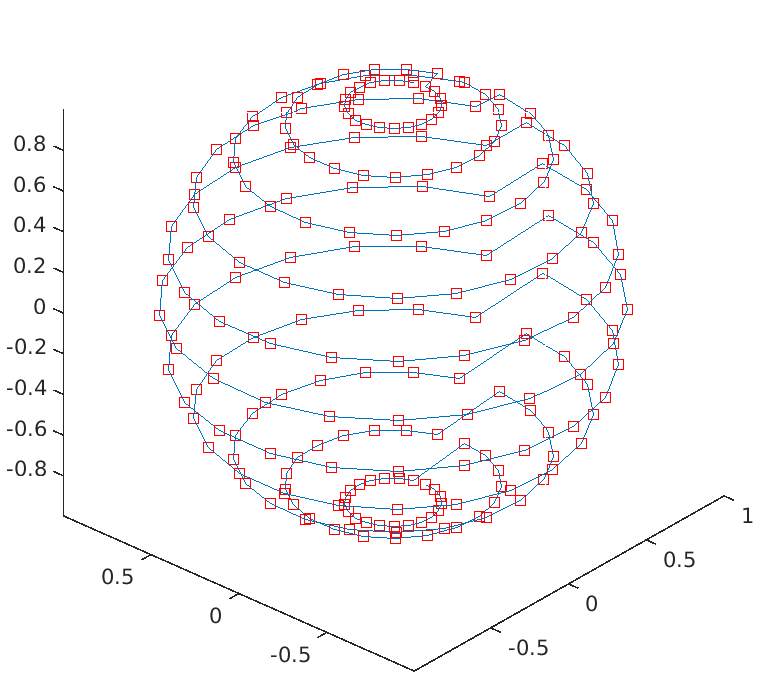
\includegraphics[height=0.4\textheight]{sphere}
  \caption{Représenation de la sphère pour $L=10$.}
  \label{fig:sph}
\end{figure}

Nous allons vérifier cette quadrature sur les harmoniques sphériques
\[
  Y_{lm}(\hs) = \sqrt{\frac{(2l+1)(l-m)!}{4\pi(l+m)!}} P^m_l(\cos(\theta)) e^{im\varphi} \quad \forall l \geq 0,~ \forall -l \leq m \leq l
\]
dont on connaît la formule d'intégration théorique
\[
  \int_{S^2} Y_{lm} = \sum_{i,j} w^\varphi_i w^\theta_j Y_{lm}(\theta_j, \varphi_i) = \quad
  \begin{cases}
    2\sqrt{\pi} & \text{si } l=m=0 \\
    0 & \text{sinon.}
  \end{cases}
\]
On obtient en effet les valeurs attendues avec des nombres complexes dont la norme est d'environs $10^{-16}$ pour les valeurs non nulles de
$l, m$ et est proche de $2\sqrt{\pi}$ pour $(l, m) = (0,0)$ à la précision flottante près.

Cependant, on aimerait en savoir plus sur comment se comporte la valeur de cette intégrale en fonction du $L$, choisi pour l'instant
arbitrairement. On oberve qualitativement dans un premier temps que pour un $l$ fixé et pour tout $m\in[0,l]$, il y a une valeur seuil de
$L$ à partir de laquelle la valeur de l'intégrale chute de plusieurs ordres de grandeur en passant de l'unité à $10^{-16}$. La dépendance
de ce $L_{\smbox{seuil}}$ par rapport au paramètre $l$ est tracée en \autoref{fig:L_min_l}, o\`u on peut supposer une relation
linéraire avec un coeficient d'environ $1/2$. 
\begin{figure}
  \centering
  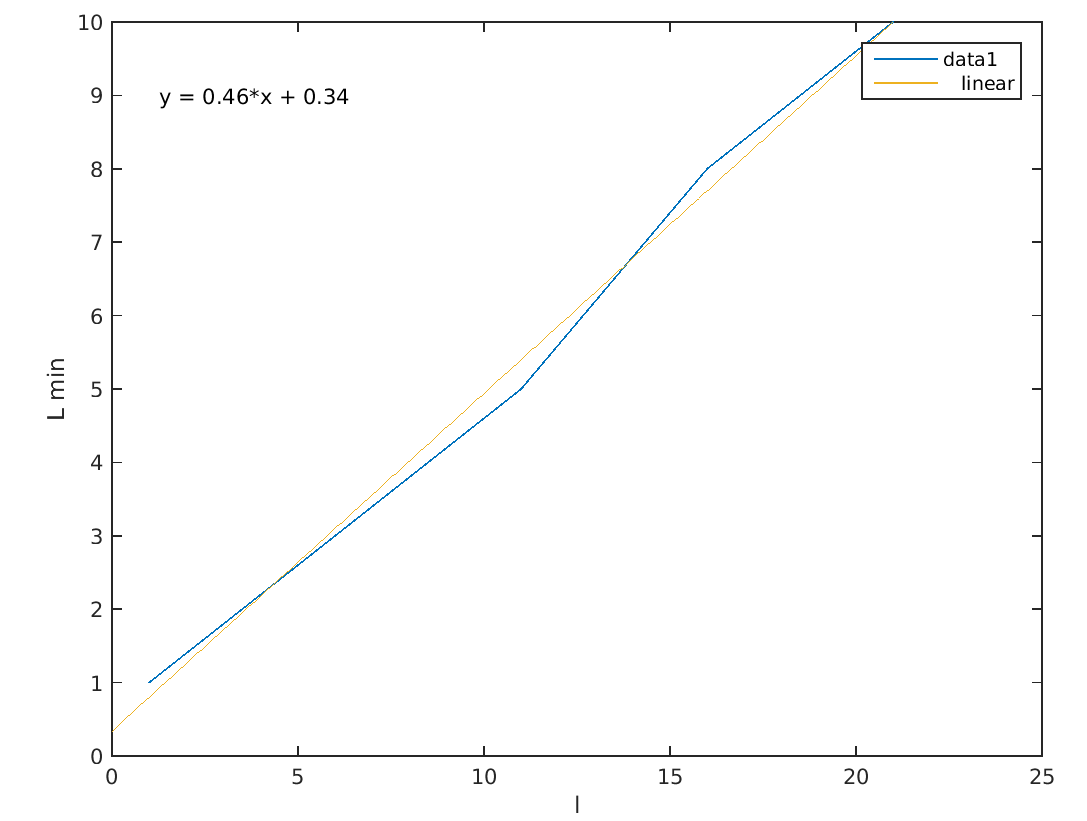
\includegraphics[height=0.4\textheight]{L_min_l}
  \caption{Valeur de $L_{\smbox{seuil}}$  à partir de laquelle l'intégrale est supposée juste en fonction de $l$.}
  \label{fig:L_min_l}
\end{figure}

On ne s'attend pas à avoir un comportement identique plus tard mais on peut espérer trouver des similarités, sinon cette étude nous à au
moins permis de savoir de quel ordre de grandeur on doit choisir $L$ pour des cas simples. 

\section{Éléments de calculs de la fonction $\lG_L$}

\begin{rmq}
  Dans la suite on note $\circ$ le produit terme à terme (aussi appelé produit de Schur).
\end{rmq}

On rappelle que les fonctions Hankel sphériques $h^{(1)}_n$ s'obtiennent à partir des fonctions de Hankel $H^{(1)}_n$ cartésiennes
implémentées dans MATLAB avec la formule
\[
  h^{(1)}_n(z) = \sqrt{\frac{\pi}{2z}}H^{(1)}_{n+1/2}(z), \quad \forall z \in \C, \forall n \in \N
\]

Le calcul vectorialisé de la valeur de $\lG_L(\hs, r_0)$ avec $N_{\hs}$ points de quadrature se fait comme suit
\begin{enumerate}
\item Créer le vecteur $F\in\C^L$ tel que $F_p = (2p+1) i^p, \forall 1\leq p \leq L $ 
\item Créer le vecteur $H\in\C^L$ tel que $H_p = h^{(1)}_p(k|r_0|)$
\item Calculer le vecteur $K\in\C^L$ tel que $K = \frac{i k}{16 \pi^2}\,F \circ H$
\item Créer la matrice $\mathbb{P}\in\mathcal{M}_{N_{\hs}\times L}(\C)$ telle que $\mathbb{P}_{sp} = P_p(\cos(\hs_s, r_0))$
\item Calculer le vecteur $G\in\C^{N_{\hs}}$ tel que $G = \mathbb{P}K$.
\end{enumerate}
Le vecteur $G$ est le résultat vectorialisé pour les tous les points de la sphère : $G_s = \lG_L(\hs_s, r_0), ~ \forall s<N_{\hs}$.


Pour vérifier que cette fonction donne de bons résultats, on les compare avec ceux de $G(r)$ pour plusieurs paramètrisations de $L,~ r_0$
et $k$.
\end{document}
%%% Local Variables:
%%% mode: latex
%%% TeX-master: t
%%% End: